\section{Design}
% Metatext

\subsection{System design}


\subsection{User Interface Design}
This section will document the design of the graphical user interface.
The user interface (UI) provides interaction methods between the user and the app\todo{solution/product? + source}.

The UI is designed to mostly comply with the Google material design guidelines \cite{materialDesign}. The material design is "\textit{bold, graphic, intentional}", according to the guidelines \cite{materialDesign}. Following the material design guidelines makes the app have a similar aesthetic and usage method as other apps on Google Play Store. The design is clean and simple in regards to colors, and the

\begin{figure}
	\centering
	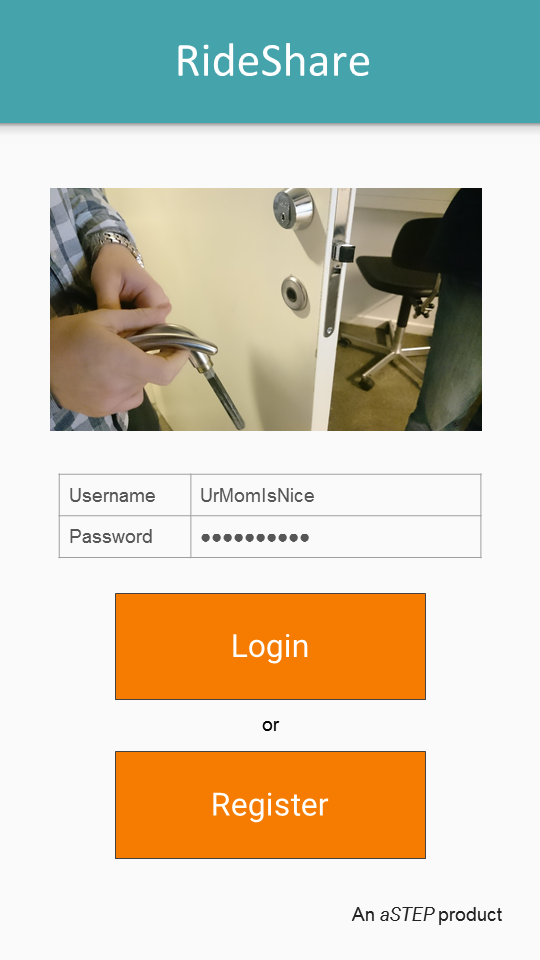
\includegraphics[width=0.25\textwidth]{figures/GUI-front.png}
	\caption{Front page with login.}
\end{figure}

\begin{figure}
	\centering
	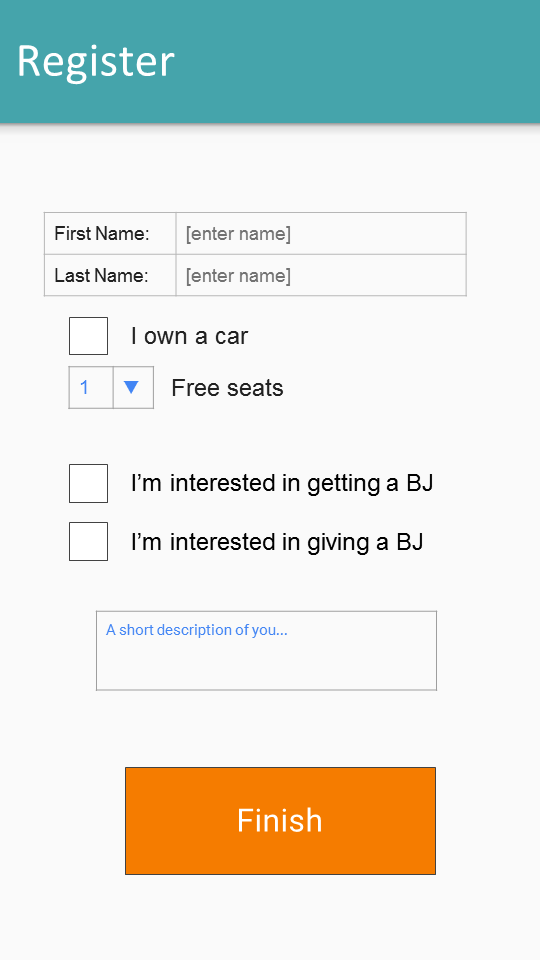
\includegraphics[width=0.25\textwidth]{figures/GUI-register.png}
	\caption{Front page with login.}
\end{figure}

\begin{figure}
	\centering
	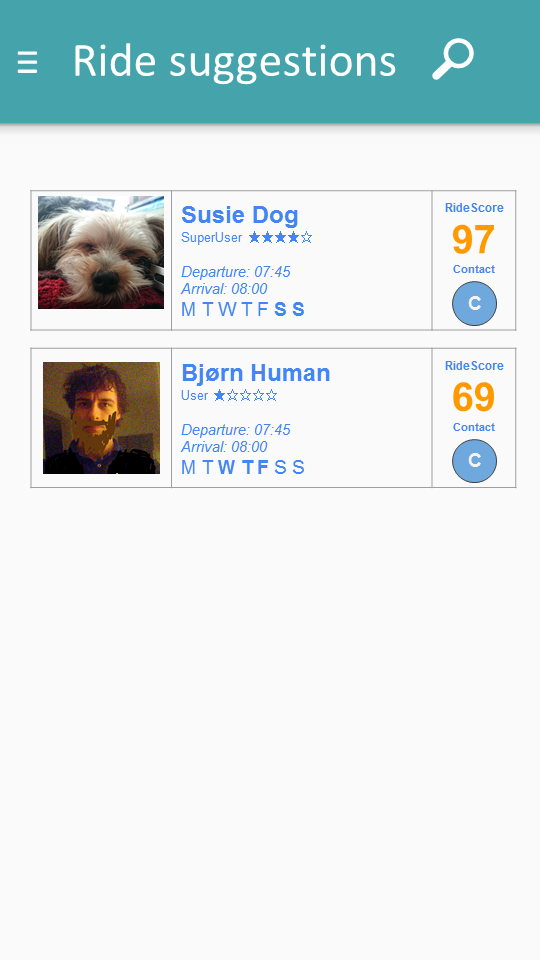
\includegraphics[width=0.25\textwidth]{figures/GUI-main.png}
	\caption{Front page with login.}
\end{figure}

\begin{figure}
	\centering
	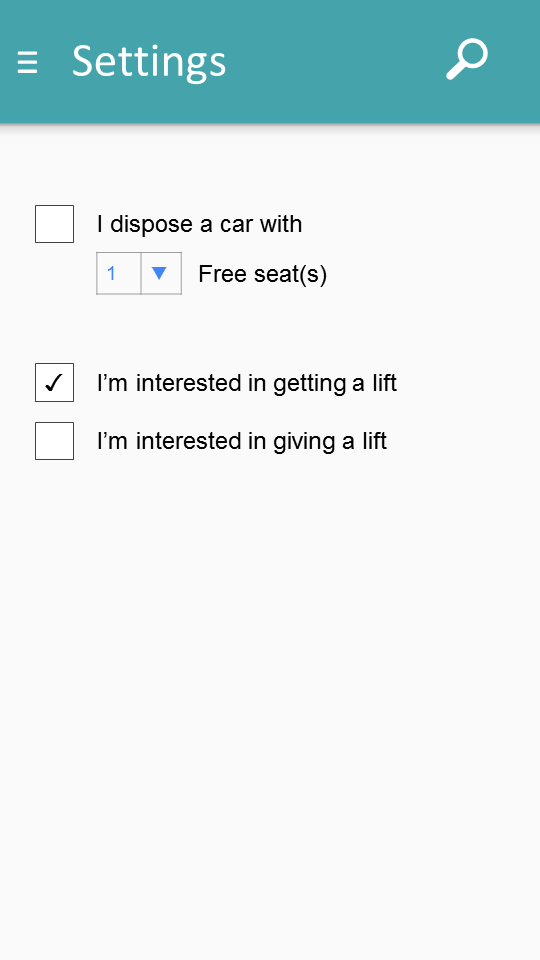
\includegraphics[width=0.25\textwidth]{figures/GUI-settings.png}
	\caption{Front page with login.}
\end{figure}
\todo{structure in table somehow}

Several interfaces are necessary to support the different parts of the app. The app needs a user interface for login, registering, presentation of matches, and a settings page, as can be seen in the figures.